\section{Basic Statistical Descriptors of Data}

\begin{frame}{Basic Statistical Descriptions of Data}
	\textbf{Motivation}:
	\begin{itemize}
		\item To better understand the data: central tendency, variation and spread.
	\end{itemize}

	\textbf{Data dispersion characteristics}:
	\begin{itemize}
		\item Median, max, min, quantiles, outliers, variance etc.
	\end{itemize}

	\textbf{Numerical dimensions correspond to sorted intervals.}\\
	\begin{itemize}
		\item Data dispersion: analyzed with multiple granularities of precision.
		\item Boxplot or quantile analysis on sorted intervals
	\end{itemize}

	\textbf{Dispersion analysis on computed measures.}\\
	\begin{itemize}
		\item Folding measures into numerical dimensions.
		\item Boxplot or quantile analysis on the transformed cube.
	\end{itemize}
\end{frame}

\begin{frame}{Measuring the Central Tendency (I)}
	\begin{itemize}
		\item \textbf{Mean}:
		      \begin{itemize}
			      \item $N$ denotes the amount of samples within the data set.
			      \item The \textbf{sample mean} is given by\\
			            \begin{equation*}
				            \bar{x} = \frac{1}{N} \sum_{i=1}^{N} x_i.
			            \end{equation*}
			      \item While the \textbf{population mean} is defined by
			            \begin{equation*}
				            \mu = \sum x \cdot p(x | \theta) \cdots.
			            \end{equation*}
		      \end{itemize}
	\end{itemize}
\end{frame}

\begin{frame}{Measuring the Central Tendency (II)}
	\begin{columns}
		\begin{column}{0.6\textwidth}
			\textbf{Median:}
			\begin{itemize}[noitemsep]
				\item The median $\tilde{x}$ minimizes the sum of absolute deviations for any $x$ of a sample $X$:
				      \begin{align}
					      \sum_{i=1}^{n} |\tilde{x}-x_i| \leq \sum_{i=1}^{n} |x-x_i|.
				      \end{align}
				      \begin{align}
					      \tilde{x} = \begin{cases}
						                  x_{\frac{N}{2}}                               & \text{if $N$ mod $2 = 0$,}    \\
						                  \frac{x_{\frac{N-1}{2}}+x_{\frac{N+1}{2}}}{2} & \text{if $N$ mod $2 \neq 0$.}
					                  \end{cases}
				      \end{align}
			\end{itemize}
		\end{column}
		\begin{column}{0.3\textwidth}  %%<--- here
			\begin{table}
				\begin{tabular}{|c|c|}
					Age      & Frequency \\ \hline
					$1-5$    & $200$     \\
					$6-15$   & $450$     \\
					$16-20$  & $300$     \\
					$21-50$  & $1500$    \\
					$51-80$  & $700$     \\
					$81-110$ & $44$
				\end{tabular}\\[0.5cm]
			\end{table}
		\end{column}
	\end{columns}
\end{frame}

\begin{frame}{Measuring the Central Tendency (III)}
	\begin{columns}
		\begin{column}{0.6\textwidth}
			\textbf{Median for interval grouped data:}
			\begin{itemize}[noitemsep]
				\item Let $n$ be the total amount of data points, $n_i$ the respective number of the $i$th group and $l_i$ or $u_i$ the lower or upper interval limit. We determine the group to which the median belongs and denote it as $m$th group. It is determined by
				      \begin{align}
					      \sum_{k=1}^{m-1}n_k < \frac{n}{2}, \; \text{but} \; \sum_{k=1}^{m} n_k \geq \frac{n}{2}.
				      \end{align}
				\item If there is no information about the underlying distribution, we just assume that data is equally distributed and use linear interpolation to estimate the median:
				      \begin{align}
					      \tilde{x} = l_m + \frac{\frac{n}{2}-\sum_{k=1}^{m-1}n_k}{n_m} \cdot (u_m-l_m).
				      \end{align}
			\end{itemize}
		\end{column}
		\begin{column}{0.3\textwidth}  %%<--- here
			\begin{table}
				\begin{tabular}{|c|c|}
					Age      & Frequency \\ \hline
					$1-5$    & $200$     \\
					$6-15$   & $450$     \\
					$16-20$  & $300$     \\
					$21-50$  & $1500$    \\
					$51-80$  & $700$     \\
					$81-110$ & $44$
				\end{tabular}\\[0.5cm]
			\end{table}
		\end{column}
	\end{columns}
\end{frame}

\begin{frame}{Measuring the Central Tendency (IV)}
	\begin{columns}
		\begin{column}{0.6\textwidth}
			\textbf{Mode:}
			\begin{itemize}[noitemsep]
				\item Value that occurs most frequently within the data set.
				\item Can be unimodal, bimodal, trimodal etc.
				\item Empirical formula:
				      \begin{align}
					      \overline{x} - \text{mode} \approx 3(\overline{x}- \tilde{x}).
				      \end{align}
			\end{itemize}
		\end{column}
		\begin{column}{0.3\textwidth}  %%<--- here
			\begin{table}
				\begin{tabular}{|c|c|}
					Age      & Frequency \\ \hline
					$1-5$    & $200$     \\
					$6-15$   & $450$     \\
					$16-20$  & $300$     \\
					$21-50$  & $1500$    \\
					$51-80$  & $700$     \\
					$81-110$ & $44$
				\end{tabular}\\[0.5cm]
			\end{table}
		\end{column}
	\end{columns}
\end{frame}

\begin{frame}{Example of Mode, Median and Mean (I)}
	\centering
	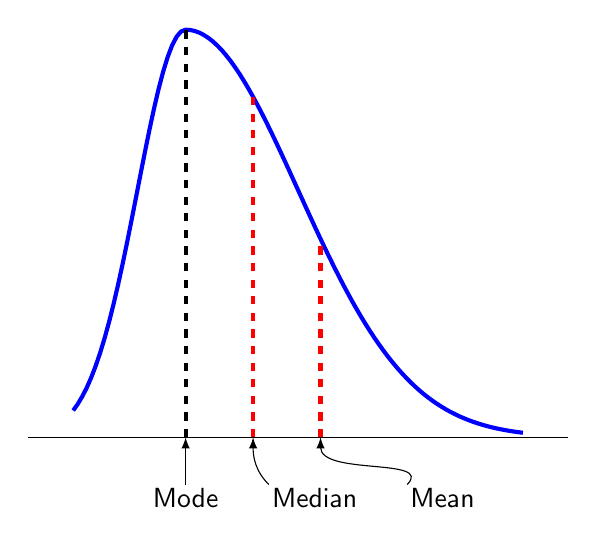
\begin{tikzpicture}[font=\sffamily,
			declare function={Gauss(\x,\y,\z,\u)=1/(\z*sqrt(2*pi))*exp(-((\x-\y+\u*(\x-\y)*sign(\x-\y))^2)/(2*\z^2));},
			every pin edge/.style={latex-,line width=1.5pt},
			every pin/.style={fill=yellow!50,rectangle,rounded corners=3pt,font=\small}]
		\begin{axis}[
				every axis plot post/.append style={
						mark=none,samples=101},
				clip=false,
				axis y line=none,
				axis x line*=bottom,
				ymin=0,
				xtick=\empty,]
			\addplot[line width=1.5pt,blue,domain=-1:3] {Gauss(x,0,0.6,-0.4)};
			\draw[line width=1.5pt,dashed, black] (0,0) -- (0,{Gauss(0,0,0.6,-0.4)});
			\draw[line width=1.5pt,dashed, red] (0.6,0) -- (0.6,{Gauss(0.6,0,0.6,-0.4)});
			\draw[line width=1.5pt,dashed, red] (1.2,0) -- (1.2,{Gauss(0.5,0,0.7,0.5)});
			\path (1.2,0) coordinate (ML) (0.6,0) coordinate (MR) (0,0) coordinate (MM);
		\end{axis}
		\draw[latex-] (ML) to[out=-90,in=45] ++ (1.1,-0.6) node[below right,inner
			sep=1pt]{Mean};
		\draw[latex-] (MR) to[out=-90,in=135] ++ (0.2,-0.6) node[below right,inner
			sep=1pt]{Median};
		\draw[latex-] (MM) --++ (0,-0.6) node[below,inner
			sep=1pt]{Mode};
	\end{tikzpicture}
	\begin{align}
		f(x \vert \mu, \sigma) = \frac{1}{\sqrt{2\pi\sigma^2}} \exp\left( - \frac{(x-\mu)^2}{2\sigma^2}\right).
	\end{align}
\end{frame}

\begin{frame}{Example of Mode, Median and Mean (II)}
	\textbf{Quartiles, outliers and boxplots:}
	\begin{itemize}
		\item \textbf{Quartiles:} {\color{blue}$\mathbf{Q}_1$} ($25^{\text{th}}$ percentile), {\color{blue}$\mathbf{Q}_3$} ($75^{\text{th}}$ percentile).
		\item \textbf{Inter quartile range:} {\color{blue}IQR} $=Q_3-Q_1$.
		\item Five number summary: min, $Q_1$, median, $Q_3$, max.
		\item \textbf{Boxplot}: ends of the box are the quartiles; \\ median is marked; add whiskers and plot outliers individually.
		\item \textbf{Outlier}: usually assigned to values higher/lower than $1.5 \cdot \text{IQR}$.
	\end{itemize}
	\textbf{Variance $\sigma^2$ and standard deviation $\sigma$}:
	\begin{itemize}
		\item Empirical sample variance: $\overline{\sigma^2} = \frac{1}{n-1} \sum_{i=1}^{n}(x_i-\overline{x})^2$
		\item Empirical population variance: $\sigma^2 = \frac{1}{N} \sum_{i=1}^{N} (x_i - \mu)^2$.
		\item Standard deviation is the square root $\sigma = \sqrt{\sigma^2}$.
	\end{itemize}
\end{frame}

\begin{frame}{Boxplot Analysis}
	\begin{center}
		\begin{tikzpicture}[scale=0.7, transform shape]
			\filldraw[fill=blue!20] (2,0) rectangle (5,1);% draw the box
			\draw (3,0) -- (3,1) node[above]{$\tilde{x}$};% draw the median
			\draw (5,0.5) -- (7,0.5);% draw right whisker
			\draw (2,0.5) -- (1,0.5);% draw left whisker
			\draw (7,0.39) -- (7,0.61);% draw vertical tab
			\draw (1,0.39) -- (1,0.61);% draw vertical tab
			\node[below] at (2,0) {$Q_1$};% label the hinge
			\node[below] at (5,0) {$Q_3$};% label the hinge
			\filldraw[ball color=yellow!80,shading=ball] (4,0.5) circle
			(0.06cm) node[above]{$\bar{x}$};% the mean
			\draw[<->] (2.3, -0.3) -- (4.7, -0.3)
			node[pos=0.5,below]{$\textsc{IQR}$}; % mark the IQR fences
			\draw[<->] (2, -0.8) -- (0,-0.8)
			node[pos=0.5,below]{$\textsc{1.5*IQR}$}; % left inner fence
			\draw[<->] (2,-1.4) -- (-2, -1.4)
			node[pos=0.5,below]{$\textsc{3*IQR}$};% left outer fence
			\draw[<->] (5, -0.8) -- (8,-0.8)
			node[midway,below]{$\textsc{1.5*IQR}$}; % right inner fence
			\draw[<->] (5,-1.4) -- (10, -1.4)
			node[pos=0.5,below]{$\textsc{3*IQR}$};% right outer fence
			%
			\node[below] at (9,0.7) {$\textbf{Outlier}$}; % mild outlier on the right
			\node[below] at (-2.4,0.7) {$\textbf{Outlier}$}; % extreme outlier on the left
			% Axis
			\draw (-3,-2) -- (11,-2);
			% Note that the snaked line is drawn to 11.1 to force
			% TikZ to draw the final tick.
			\draw[snake=ticks,segment length=1cm] (-3,-2) -- (11.1,-2);
		\end{tikzpicture}
	\end{center}
	\textbf{Five number summary of a distribution:}\\
	Minimum, $Q_1$, median, $Q_3$, maximum.
	\\[0.2cm]
	\textbf{Boxplot}:
	\begin{itemize}
		\item Data is represented with a box.
		\item The ends of the box are at the first and third quartiles, i.e. the height of the box is IQR. \\
		      The median is marked by a line within the box.
		\item Whiskers: two lines outside the box extended to minimum and maximum.
		\item Outliers: points beyond a specified outlier threshold, plotted individually.
	\end{itemize}
\end{frame}

\begin{frame}{Properties of Normal Distribution Curves}
	\begin{itemize}
		\item \textbf{The normal distribution:}
		      \begin{itemize}
			      \item From $\mu - \sigma$ to $\mu + \sigma$: contains about $68\%$ of the measurements.
			            \begin{itemize}
				            \item $\mu$: mean,
				            \item $\sigma$: standard deviation.
			            \end{itemize}
			      \item From $\mu - 2 \sigma$ to $\mu + 2\sigma$: contains about $95\%$ of the surface under the curve.
			      \item $\mu-3\sigma$ to $\mu + 3\sigma$: contains about $99.7\%$ of the surface under the curve.
		      \end{itemize}
	\end{itemize}
	\vspace{0.2cm}
	\centering
	\begin{tikzpicture}
		\begin{axis}[
				no markers, domain=-3:3, samples=100,
				axis lines*=left, xlabel=$x$, ylabel=$y$,
				height=3.5cm, width = 5cm,
				xtick={-3,-2,-1,0,1,2,3}, ytick=\empty,
				enlargelimits=false, clip=false, axis on top,
				grid = major
			]
			\addplot [fill=blue!20, draw=none, domain=-1:1] {gauss(0,1)} \closedcycle;
			\addplot [very thick,blue!50!black] {gauss(0,1)};
			\node[below] at (0,0.15) {$\approx 66 \%$};
		\end{axis}
	\end{tikzpicture}
	\hspace{0.2cm}
	\begin{tikzpicture}
		\begin{axis}[
				no markers, domain=-3:3, samples=100,
				axis lines*=left, xlabel=$x$, ylabel=$y$,
				height=3.5cm, width = 5cm,
				xtick={-3,-2,-1,0,1,2,3}, ytick=\empty,
				enlargelimits=false, clip=false, axis on top,
				grid = major
			]
			\addplot [fill=blue!20, draw=none, domain=-2:2] {gauss(0,1)} \closedcycle;
			\addplot [very thick,blue!50!black] {gauss(0,1)};
			\node[below] at (0,0.15) {$\approx 95 \%$};
		\end{axis}
	\end{tikzpicture}
	\hspace{0.2cm}
	\begin{tikzpicture}
		\begin{axis}[
				no markers, domain=-3:3, samples=100,
				axis lines*=left, xlabel=$x$, ylabel=$y$,
				height=3.5cm, width = 5cm,
				xtick={-3,-2,-1,0,1,2,3}, ytick=\empty,
				enlargelimits=false, clip=false, axis on top,
				grid = major
			]
			\addplot [fill=blue!20, draw=none, domain=-2.97:2.97] {gauss(0,1)} \closedcycle;
			\addplot [very thick,blue!50!black] {gauss(0,1)};
			\node[below] at (0,0.15) {$\approx 99.7 \%$};
		\end{axis}
	\end{tikzpicture}
	\hspace{0.2cm}
\end{frame}

\begin{frame}{Visualization of Basic Statistical Descriptions}
	\begin{itemize}
		\item \textbf{Boxplot}: Visualization of five number summary.
		\item \textbf{Histogram}: $x$-axis are values, $y$-axis represent frequencies.
		\item \textbf{Quantile plot}: Each value $x_i$ is paired with some $q_i$ indicating that approximately $q_i \cdot 100 \%$ of data are $\leq x_i$.
		\item \textbf{Quantile-quantile (q-q) plot}: Graphs the quantiles of one univariate distribution against the corresponding quantiles of another.
		\item \textbf{Scatter plot}: Each pair of values is a pair of coordinates and plotted as points in the plane.
	\end{itemize}
\end{frame}

\begin{frame}{Histogram Analysis}
	\begin{itemize}
		\item \textbf{Histogram}: Visualization of tabulated frequencies, shown as bars.
		\item It shows what proportion of cases fall into each of several categories.
		\item Differs from a $\textbf{bar chart}$ in that it is the \emph{area} of the bar that denotes the value, not the height as in bar charts, a crucial distinction when the categories are not of uniform width.
		\item The categories are usually specified as non-overlapping intervals of some variable. The categories (bars) must be adjacent.
	\end{itemize}\vspace{0.2cm}
	\centering
	\begin{tikzpicture}
		\begin{axis}[
				yticklabel style={/pgf/number format/fixed},
				scaled y ticks = false,
				minor y tick num={1},
				xtick pos=left,
				legend cell align = left,
				legend style={draw=none},
				xlabel = {group size},
				ylabel = {ratio}
			]
			\addplot[blue,ybar,fill, fill opacity=0.3, bar width = 0.8,] table {data.dat};
			\addplot[red, line width = 1,domain=1:40,samples=100] {1/(x*sqrt(2*pi)*\plots)*exp(-(ln(x)-\plotm)^2/(2*\plots^2))};
			\legend{empirical,lognormal fit}
		\end{axis}
	\end{tikzpicture}
\end{frame}

\begin{frame}{Histograms Often Tell More than Boxplots}
	The two histograms shown below may have the same boxplot representation, thus the same values for min, $Q_1$, median, $Q_3$ and for the max. But they have rather different underlying distributions.\\[1cm]
	\centering
	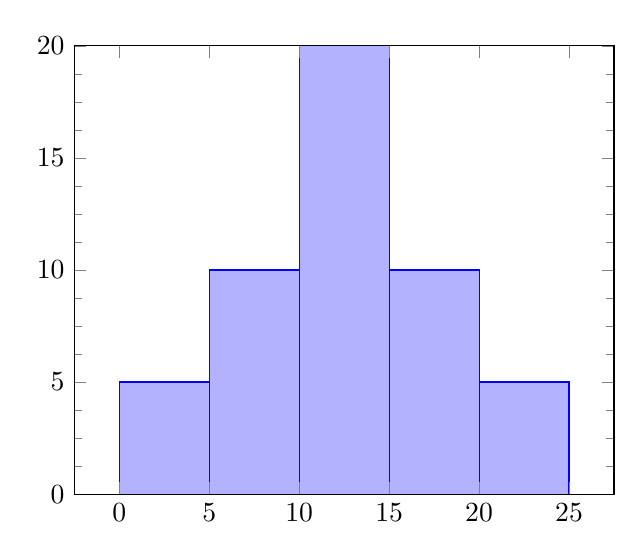
\begin{tikzpicture}
		\begin{axis}[
				ymin=0, ymax=20,
				minor y tick num = 3,
				area style,
			]
			\addplot+[ybar interval,mark=no] plot coordinates {(0, 5) (5, 10) (10, 20) (15,10) (20,5) (25,5)};
		\end{axis}
	\end{tikzpicture}
	\hspace{0.5cm}
	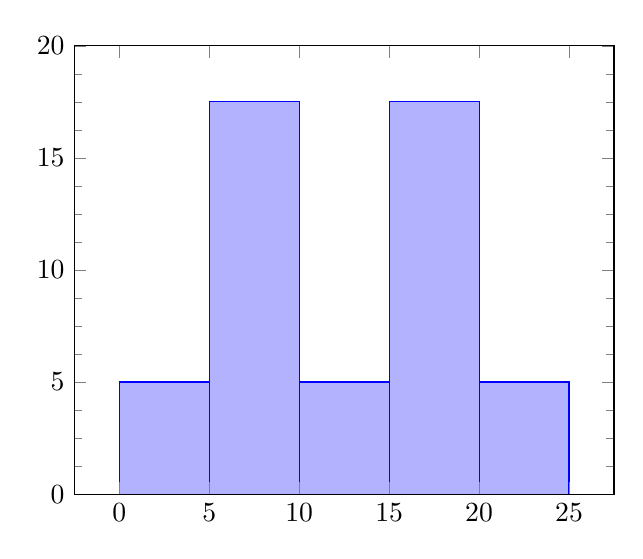
\begin{tikzpicture}
		\begin{axis}[
				ymin=0, ymax=20,
				minor y tick num = 3,
				area style,
			]
			\addplot+[ybar interval,mark=no] plot coordinates {(0, 5) (5, 17.5) (10, 5) (15,17.5) (20,5) (25,5)};
		\end{axis}
	\end{tikzpicture}
\end{frame}

\begin{frame}{Quantile Plot}
	\textbf{Displays all of the data.}\\
	A quantile plot allows the user to assess both the overall behaviour and unusual occurrences.\\[0.5cm]
	\textbf{Plots quantile information.}\\
	For some data point $x_i$, sorted in increasing order, $q_i$ indicates that approximately $q_i \cdot 100 \%$ of the data are below or equal to the value of $x_i$.\\[0.2cm]
	\centering
	\begin{tikzpicture}[
			declare function={norm(\x)=\x*\x/200;},
		]
		\begin{axis}[
				ylabel={Unit price in \$},
				xlabel={q-value},
			]
			\addplot[color=black, thick] table [x index=0, y index=0, x expr = \coordindex/100, y expr=norm(\coordindex)] {\sorted};
		\end{axis}
	\end{tikzpicture}
\end{frame}

\begin{frame}{Quantile-quantile ($q-q$) Plot}
	\begin{itemize}
		\item Graphs the quantiles of one univariate distribution against the corresponding quantiles of another.
		\item View: Do these two distributions differ?\\
		      Example shows unit price of items sold at Branch $1$ vs. branch $2$ for each quantile.  Unit prices of items sold at branch $1$ tend to be lower than those at branch $2$.
	\end{itemize}\vspace{0.5cm}
	\centering
	\begin{tikzpicture}[
			declare function={norm(\x)=2*\x;},
		]
		\begin{axis}[
				ylabel={Branch 2 (unit price in \$)},
				xlabel={Branch 1 (unit price in \$)},
			]
			\addplot [only marks, mark=*] table [x index=0, y index=0, y expr=norm(\coordindex)] {\sorted};
			\draw[black, thick] (0,0) -- (200,200);
		\end{axis}
	\end{tikzpicture}
\end{frame}

\begin{frame}{Scatter Plots}
	Provides a first look at \textbf{bivariate data} to see clusters of points, outliers or similar.\\
	Each pair of values is treated as a pair of coordinates and plotted as points in the plane.\\[0.5cm]
	\centering
	\includegraphics[height=3cm]{img/scatterplot.pdf}
\end{frame}

\begin{frame}{Data Profiling}
	\begin{itemize}
		\item \textbf{More from the database perspective.}
		\item \textbf{Derive metadata such as:}
		      \begin{itemize}
			      \item Data types and value patterns.
			      \item Completeness and uniqueness of columns.
			      \item Keys and foreign keys.
			      \item Occasionally functional dependencies and association rules.
			      \item Discovery of inclusion dependencies and conditional functional dependencies.
		      \end{itemize}
		\item \textbf{Statistics:}
		      \begin{itemize}
			      \item Number of null values and distinct values in a column.
			      \item Data types.
			      \item Most frequent patterns of values.
		      \end{itemize}
	\end{itemize}
\end{frame}
